\section{Analysis}
\label{sec:analysis}

\subsection{Feasability of DNS request linking}
\fixme{rerun all experiments with more sites}
% flow:
% - we get signal (precision), confirming what kNN says
% - signal depends on pct of exit bandwidth, but improve precision
% 	already at small pct (but big impact on recall)
% - signal depends on monitored sites' popularity
% - WF less good at annoying base rate -> precision goes down
% 	with 1:1 ratio, the base rate is 0.5 when testing.
%  We flip the base rate to 10*100/100*1000 = 0.01

We perform 10-fold cross-validation for all of our experiments in the open
world setting. We monitor 1000 sites with 100 instances each and
$100*1000$ unmonitored sites unless otherwise stated.
\fixme{data collection}
Note the 1:1 ratio between monitored traces and unmonitored traces,
ensuring that for the classifier there is equal probability in the testing
phase that a trace is a monitored or unmonitored site.
In other words, the \emph{base rate} is 0.5 in our experiments.
Furthermore, for all experiments we define an \emph{offset} that specifies
which sites on Alexa are monitored. An offset of 0 means that Alexa sites
[1,1000] are monitored and Alexa [1001,101000] unmonitored. An offset of 100
means that Alexa sites [101,1100] are monitored, and Alexa [1,100] and
[1101,10100] unmonitored.
We never monitor an unmonitored site or vice versa. How popular monitored sites
are is a key factor in the effectiveness of our attacks.
% note: base rate is per user, while popularity in Alexa for DNS observations
% is world-wide

Figure~\ref{fig:wfdns:torpct} shows the recall and precision for our WF+DNS
attacks as a function of the percentage of observed Tor exit bandwidth by the
attacker at offset $10^5$. We show Wa-kNN with $k=2$ and $k=4$.
\fixme{Recall measures the probability that a visit to a monitored page will
be detected, while precision measures the probability that a classification by
the classifier of a visit to a monitored site (positive test outcome) is the
correct one. Note that precision captures the base rate in an experiment.}
For recall, regardless of $k$, both \texttt{ctw} and \texttt{hp} are
significantly impacted by the percentage of exit bandwidth observed by the
attacker. An attacker cannot identify a monitored site in the DNS data that
she does not see.
%Already at 5\% of
%\fixme{snapshotsim bug or something else?}
For precision we see a significant gain at low percentages with a small steady
gain as the observed exit bandwidth increases. As we increase $k$ from 2 to 4
we trade decreased recall for increased precision in the \texttt{wf} attack
and the relative gain in precision is much smaller. Since we are already at
such high precision ($>0.9$) this is expected.

\begin{figure}[t]
\centering
\subfigure[Recall]{
	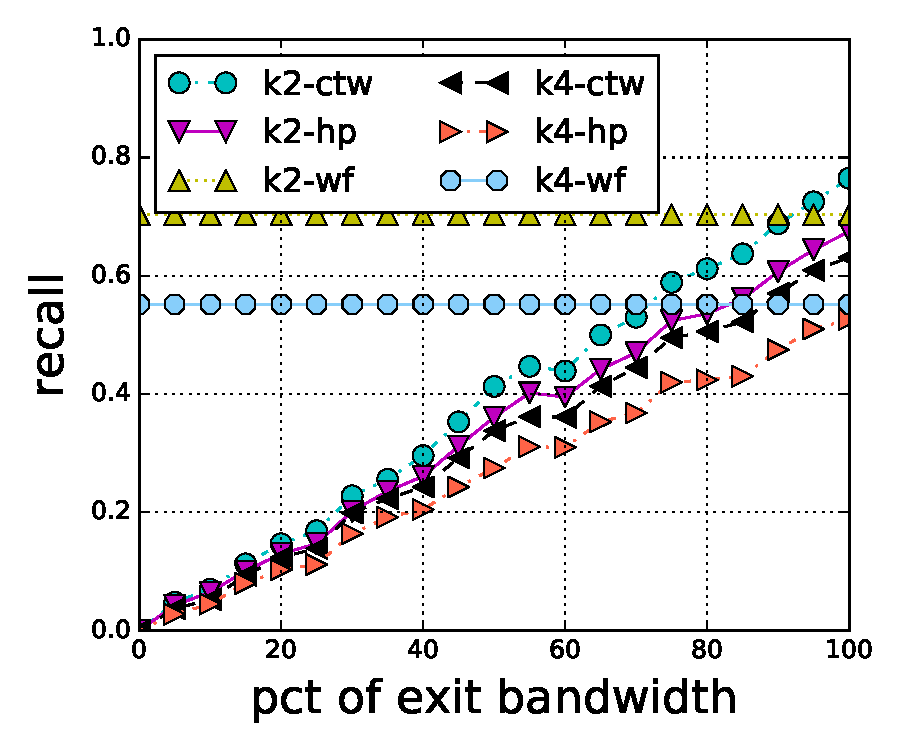
\includegraphics[width=0.466\linewidth]{figures/wfdns/pct/10x100+1000-dns2site-alexa10000-recall}
    \label{fig:wfdns:torpct:recall}
}
\subfigure[Precision]{
	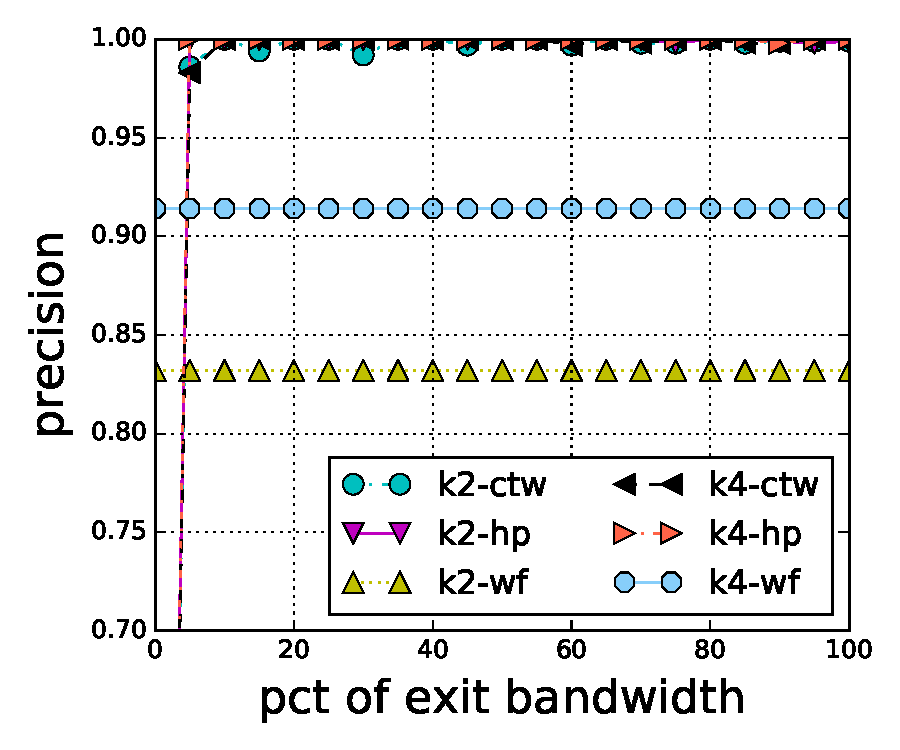
\includegraphics[width=0.466\linewidth]{figures/wfdns/pct/10x100+1000-dns2site-alexa10000-precision}
    \label{fig:wfdns:torpct:precision}
}
\caption{10x100+1k-dns2site-alexa10k}
\label{fig:wfdns:torpct}
\end{figure}


Figure~\ref{fig:wfdns:offsets} shows recall and precision at 50 percentage of
observed Tor exit bandwidth as a function of the offset. For monitored sites in
Alexa top-1000 we see no notable difference between any of the attacks in either
recall or precision: popular sites are virtually always visited by some Tor user
so they always show up in the attackers DNS data. At $10^4$ and onwards we see
the different attacks diverging: recall goes down and precision goes up,
indicating that our attacks can use the DNS data to augment precision.
DNS data is only useful for an attacker for less popular websites, such as
\url{wikileaks.org} at Alexa rank 10808.
% we should see a smaller match, hopefully there in bigger dataset


\begin{figure}[t]
\centering
\subfigure[Recall]{
	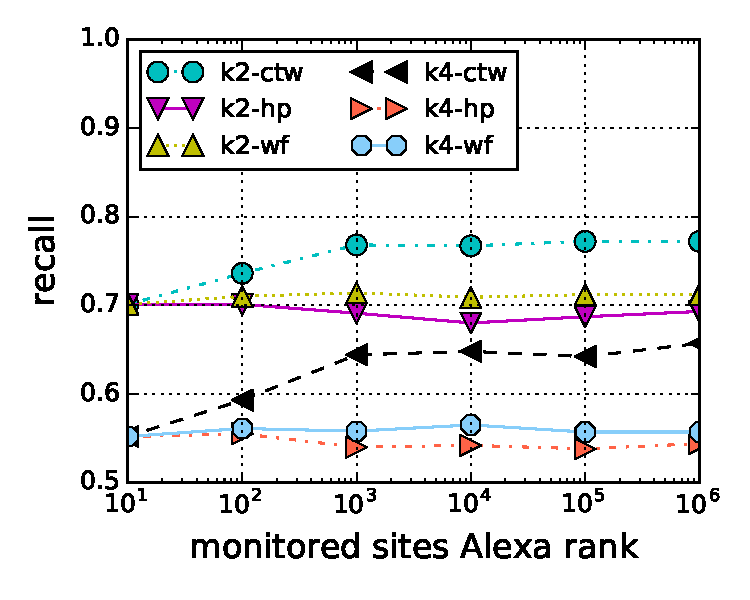
\includegraphics[width=0.466\linewidth]{figures/wfdns/offsets/10x100+1k-offsets-100pct-recall}
    \label{fig:wfdns:offsets:recall}
}
\subfigure[Precision]{
	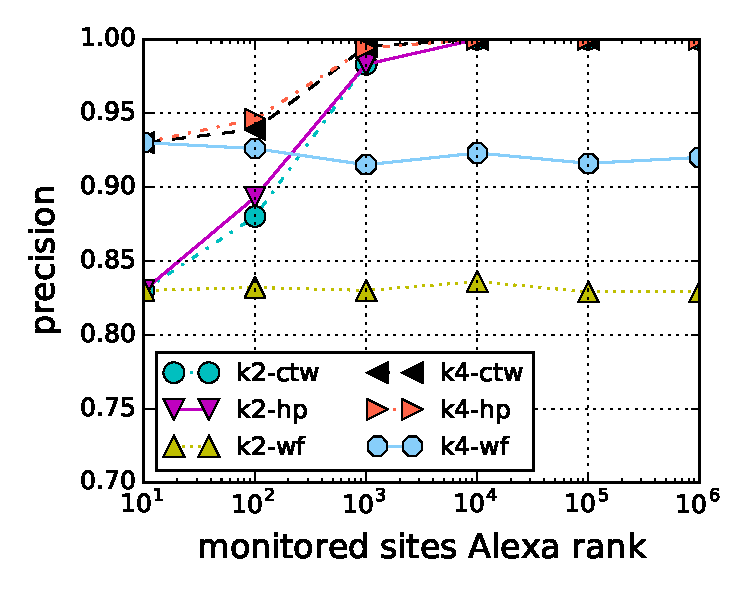
\includegraphics[width=0.466\linewidth]{figures/wfdns/offsets/10x100+1k-offsets-100pct-precision}
    \label{fig:wfdns:offsets:precision}
}
\caption{10x100+1k-offsets at 100 percentage of Tor exit bandwidth.}
\label{fig:wfdns:offsets}
\end{figure}

% impact of:
% - fixing Tor TTL bug,
% - different min/max TTLs

% limitation: webSITES, not wePAGES in our analysis + what we get from DNS.
